\documentclass{../../../yukibook.cls/yukibook}

\begin{document}

\yukibook{Sistemas Operativos \linebreak en red} 	% Title
  {Rubén Gómez}  % Author
  {2021-2022}    % Year
  {Técnico en Sistemas microinformáticos y redes} % Name of degree
  {\textquote{A very good phrase for a very good book}}	% catch phrase
  {The phrase's author}	% the phrase's author
  {img/cover.png}

%--------------------------------------------------------------------------
% Start your parts, chapters and sections here
%--------------------------------------------------------------------------

%\part{Part 1}

\chapter{Introducción a GNU/Linux}
\section{Un poco de historia}
Para conocer cómo nació el movimiento GNU y el kernel Linux debemos conocer un poco de historia de la informática y cómo evolucionó en los primeros años.

\subsection{El nacimiento de Unix}

\begin{description}
\item[1964-1969]Los laboratorios \textbf{Bell} empiezan un proyecto con el \textbf{MIT} (Instituto Tecnológico de Massachusetts) y \textbf{General Electric} para desarrollar un sistema de \textbf{tiempo compartido} (“time-sharing computing”): se llamaría \textbf{Multics} (Multiplexed Information and Computing Service). 

Hasta este momento, los sistemas utilizados eran de un único proceso, la CPU no era compartida por múltiples procesos sino que se ejecutaba por lotes (se les mandaba los procesos a ejecutar y se ejecutaban en orden).

Multics obtuvo licencia libre en el 2007. En Diciembre del 2016 salió la última versión 12.6f.

\itemimage{1969}{r}{0.33}
  {img/Ken_Thompson_and_Dennis_Ritchie--1973.jpg}
  {\href{https://en.wikipedia.org/wiki/Ken_Thompson}{Ken y Dennis . Origen: Wikipedia}}
  {
  Uno de los desarrolladores de Multics, \href{https://en.wikipedia.org/wiki/Ken_Thompson}{Ken Thompson}, decidió escribir su propio sistema operativo. Ken Thompson es conocido también por crear el lenguaje de programación \textbf{B}, el sistema de codificación de caracteres UTF-8 y el lenguaje de programación Go, entre otras cosas.

A Ken Thompson se le une \href{https://en.wikipedia.org/wiki/Dennis_Ritchie}{Dennis Ritchie} y otros, y empiezan a programar un sistema de ficheros jerárquico, el concepto de procesos de computación, ficheros de dispositivos, un intérprete de comandos, … El resultado de lo programado era más pequeño y simple que Multics, lo que se convertiría en Unix. En Agosto ya tendrían el sistema operativo, se auto-gestiona,  tenía un assembler, un editor y una shell de comandos.

Dennis Ritchie es conocido también por crear junto con Ken el lenguaje de programación \textbf{C} (aparece por primera vez en 1972).
}


\item[1970]En ese momento el nuevo sistema operativo se llamaba \textbf{Unics} (\textit{Uniplexed Information and Computing Service}, un juego de palabras en contraposición a  Multics). No tenían todavía dinero de la organización en el desarrollo (era desarrollado por los programadores) y tampoco era multitarea todavía.

A finales de año el sistema ya era conocido como \textbf{UNIX}, y se había portado a la máquina PDP-11.

\textbf{Las primeras versiones de Unix incluían el código fuente} para que las universidades lo pudiesen modificar y así poder extenderlo a sus necesida des.


\item[1971]El sistema se empieza a hacer complejo y como querían que más usuarios lo usasen, crean el sistema de manuales que es utilizado hoy en día (mediante el comando \textbf{"man"}).

\begin{center}
  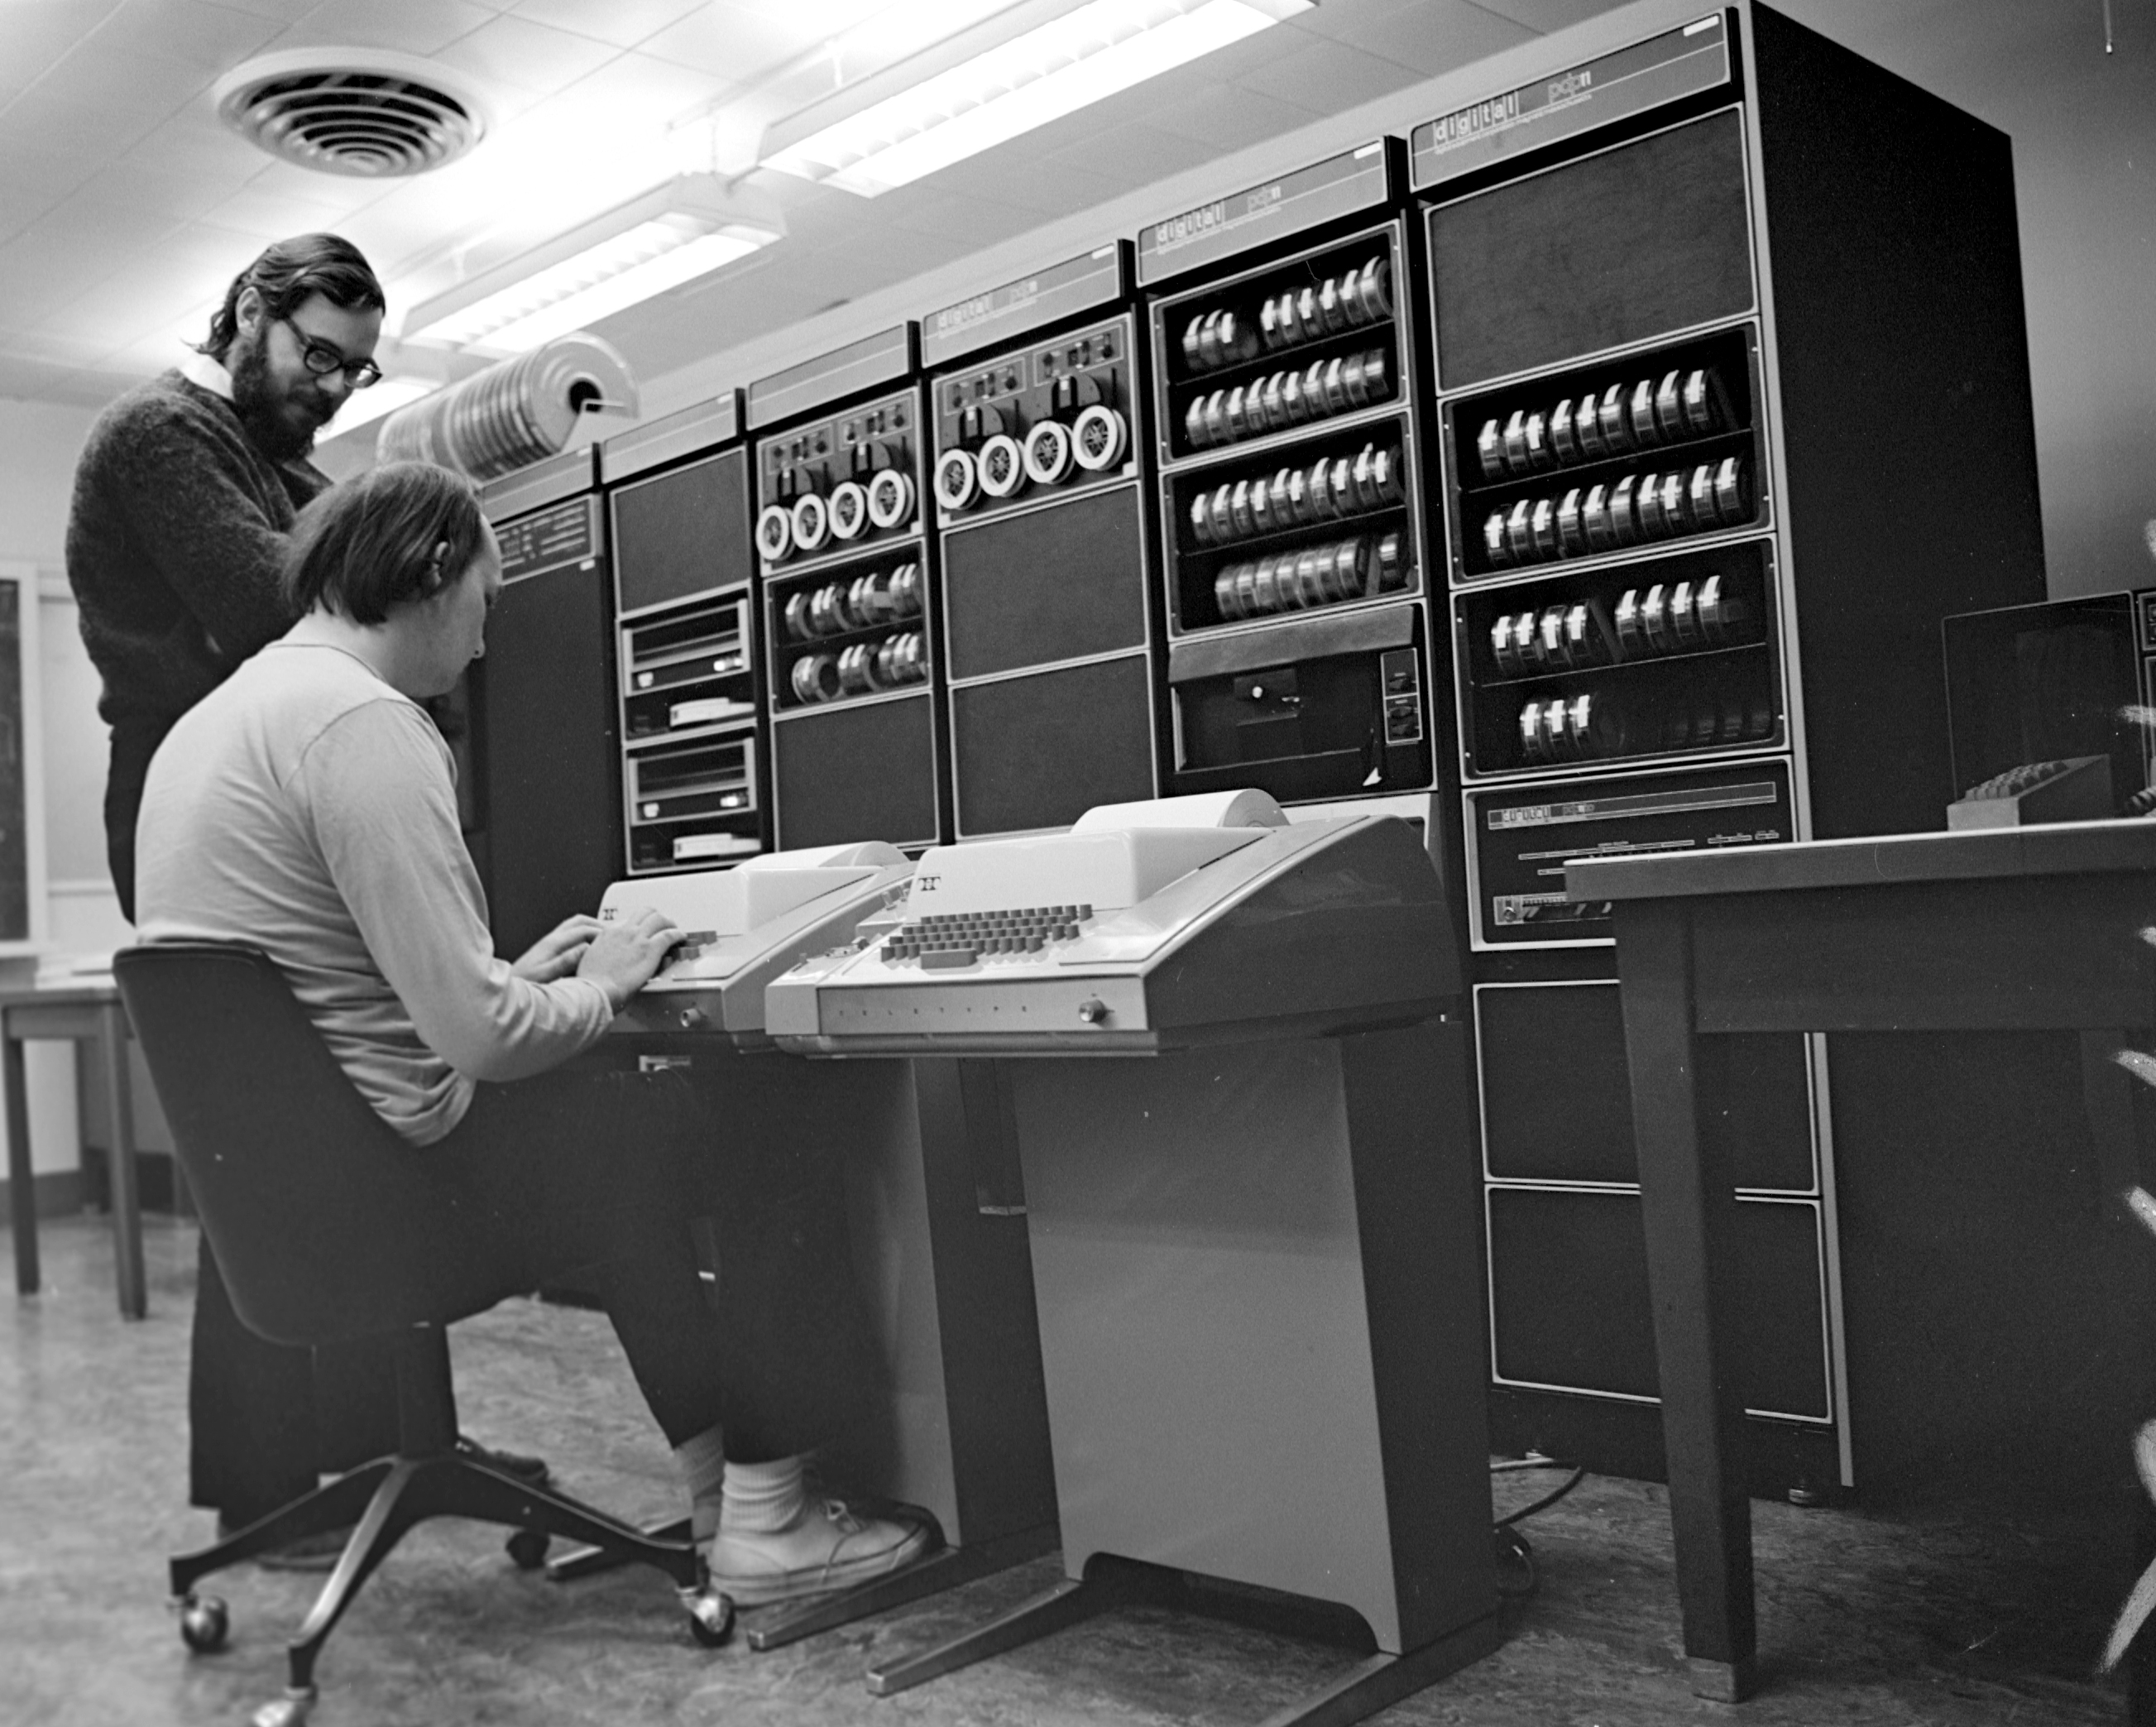
\includegraphics[width=0.8\linewidth]{img/Ken_Thompson_(sitting)_and_Dennis_Ritchie_at_PDP-11_(2876612463).jpg}
  \vspace{-10pt}\captionof{figure}{\href{https://en.wikipedia.org/wiki/Ken_Thompson}{Dennis Ritchie y Ken Thompson. Origen: Wikipedia}}\vspace{-13pt}
\end{center}


\item[1973]La versión 4 del sistema es reescrita completamente en C. Hasta este momento el sistema había estado escrito en ensamblador, por lo que no era portable entre distintos tipos de máquinas, aunque la primera versión portada a otra plataforma fue en 1978. Se cree que había “más de 20” instalaciones del sistema.

\item[1974]La versión 5 se licencia para ser utilizada en \textbf{instituciones educativas}. 

\item[1975]La versión 6 se licencia para poder ser utilizadas por empresas por \$20.000 de la época.

\item[1977]La universidad de Berkeley lanza su primera versión de Unix bajo la Berkeley Software Distribution (BSD).

\item[1979]Con la salida de Unix v7, se comienza a portar a los distintos ``microordenadores'' de la época y a los distintos microprocesadores (Motorola 68000, Intel 8086, … ).

\item[1980]Microsoft anuncia su primer Unix para microcomputadoras de 16 bits (Xenix).
\end{description}

\subsection{El nacimiento de GNU (GNU's Not Unix}
\begin{description}

\item[1971]\href{https://en.wikipedia.org/wiki/Richard_Stallman}{Richard Stallman} comienza su carrera en el MIT en el laboratorio de inteligencia artificial.

Es conocido no sólo por el movimiento GNU, si no también por crear GCC y Emacs entre otra gran cantidad de software.

En esa época el software se distribuía de manera abierta para poder ser modificado. Lo habitual era realizar modificaciones para mejorar el software y distribuirlo entre compañeros y universidades.

\itemimage{1982}{r}{0.25}
  {img/Richard_Stallman_2016_Talk_in_Madrid_06.jpg}
  {\href{https://commons.wikimedia.org/wiki/File:Richard_Stallman_2016_Talk_in_Madrid_06.jpg}{Richard Stallman: Wikimedia}}
  {
Richard Stallman quiere modificar el firmware de unas impresoras y el fabricante le pide que firme un acuerdo de no divulgación si le enseñan el código. Esto hace que Stallman se enfurezca y es cuando decide que la situación actual debe cambiar y volver al sistema de intercambio de software anterior.

\item[1983] Se anuncia el nacimiento del proyecto \textbf{GNU}, cuya finalidad es la de construir un sistema operativo completamente libre, compatible con Unix. La idea es dar a los usuarios la libertad y el control de sus ordenadores.

\item[1985] Se lanza el \href{https://www.gnu.org/gnu/manifesto.es.html}{manifiesto GNU}, y ya cuenta con un editor de texto (Emacs), compilador de C, una shell, varias utilidades … El núcleo inicial todavía no es funcional.
}

 

\item[1986]
Richard Stallman escribe y publica la definición de lo que es Free Software (Software Libre) a través de la \href{https://es.wikipedia.org/wiki/Free_Software_Foundation}{Free Software Foundation}.

\begin{tcolorbox}[title=Aclarando la palabra ``free'':]
\center
\textbf{The word ``free'' in our name does not refer to price; it refers to freedom.}

La palabra ``free'' no se refiere a gratis, si no que se refiere a libertad.
\end{tcolorbox}

Más adelante veremos a qué se refiere sobre libertad en el software.

\end{description}

\end{document}
